\documentclass[11pt, dvipsnames, handout]{beamer}
\newtoggle{full}
\settoggle{full}{true}

\newtoggle{covered}
\settoggle{covered}{false}

\newtoggle{presentable}
\settoggle{presentable}{false}

\newtoggle{dualscreen}
\settoggle{dualscreen}{false}

\usepackage{pgfplots}
%\pgfplotsset{compat = newest}

\usepackage{pgfpages}

\setbeamertemplate{note page}{\pagecolor{yellow!5}\vfill \insertnote \vfill}
\usepackage{collect}
\definecollection{notes}
\newcounter{notestaken}

\usepackage{xpatch}

\usepackage{ulem}

\usepackage[framemethod=tikz]{mdframed}

\usepackage{scalerel}
\usepackage{calc}

%\usepackage{enumitem}
\setlength\fboxsep{.2em}

\usepackage{graphicx} % Allows including images
\usepackage{booktabs} % Allows the use of \toprule, \midrule and \bottomrule in tables

\xpatchcmd{\itemize}
  {\def\makelabel}
  {\setlength{\itemsep}{0.65 em}\def\makelabel}
  {}
  {}


\xpatchcmd{\beamer@enum@}
  {\def\makelabel}
  {\setlength{\itemsep}{0.65 em}\def\makelabel}
  {}
  {}


%\makeatletter
%\renewcommand{\itemize}[1][]{%
%  \beamer@ifempty{#1}{}{\def\beamer@defaultospec{#1}}%
%  \ifnum \@itemdepth >2\relax\@toodeep\else
%    \advance\@itemdepth\@ne
%    \beamer@computepref\@itemdepth% sets \beameritemnestingprefix
%    \usebeamerfont{itemize/enumerate \beameritemnestingprefix body}%
%    \usebeamercolor[fg]{itemize/enumerate \beameritemnestingprefix body}%
%    \usebeamertemplate{itemize/enumerate \beameritemnestingprefix body begin}%
%    \list
%      {\usebeamertemplate{itemize \beameritemnestingprefix item}}
%      {%
%        \setlength\topsep{1em}%NEW
%        \setlength\partopsep{1em}%NEW
%        \setlength\itemsep{1em}%NEW
%        \def\makelabel##1{%
%          {%
%            \hss\llap{{%
%                \usebeamerfont*{itemize \beameritemnestingprefix item}%
%                \usebeamercolor[fg]{itemize \beameritemnestingprefix item}##1}}%
%          }%
%        }%
%      }
%  \fi%
%  \beamer@cramped%
%  \raggedright%
%  \beamer@firstlineitemizeunskip%
%}
%
%
%
%
%
%\makeatother

%\setlist[beamer@enum@]{topsep=1 em}
%\let\origcheckmark\checkmark %screw you dingbat
%\let\checkmark\undefined %screw you dingbat
%\usepackage{dingbat} 
%\let\checkmark\origcheckmark %screw you dingbat






%\usepackage{fontawesome}

\usepackage{mathtools}
\usepackage{etoolbox, calculator}

\usepackage{xcolor}
\usepackage{tikz}
\usetikzlibrary{arrows.meta}
\usetikzlibrary{calc}
\usepackage[nomessages]{fp}
\usepackage{transparent}
\usepackage{accsupp}
%\usepackage{color, xcolor}

%colorblind-friendly palette
%\definecolor{dblue}{RGB}{51,34,136}
\definecolor{lblue}{RGB}{136,204,238}
%\definecolor{green}{RGB}{17,119,51}
\definecolor{tan}{RGB}{221,204,119}
%\definecolor{mauve}{RGB}{204,102,119}

\usepackage{tcolorbox}



\usepackage{xifthen}
\usepackage{nicefrac}
\usepackage{amsmath}
\usepackage{amsthm}
\usepackage{amssymb}
\theoremstyle{definition}
\newtheorem*{define}{Definition}
\newtheorem*{recall}{Recall}


\DeclareMathOperator{\tr}{tr}

\usepackage{multicol}
%\setlength{\columnsep}{1cm}

\usepackage{tablists, amsmath,vwcol, cancel, polynom}
\usetikzlibrary{shapes, patterns, decorations.shapes}
%\usepackage{tikzpeople}
\tikzstyle{vertex}=[shape=circle, minimum size=2mm, inner sep=0, fill]
\tikzstyle{opendot}=[shape=circle, minimum size=2mm, inner sep=0, fill=white, draw]

% common math quick commands
\newcommand{\nicedd}[2]{\nicefrac{\text{d}#1}{\text{d}#2}}
\newcommand{\dd}[2]{\dfrac{\text{d}#1}{\text{d}#2}}
\newcommand{\pd}[2]{\dfrac{\partial #1}{\partial#2}}
\renewcommand{\d}[1]{\text{d}#1}
\newcommand{\ddn}[3]{\dfrac{\text{d}^{#3}#1}{\text{d}#2^{#3}}}
\newcommand{\pdn}[3]{\dfrac{\partial^{#3}#1}{\partial#2^{#3}}}
\newcommand{\p}[0]{^{\prime}}
\newcommand{\pp}[0]{^{\prime\prime}}
\newcommand{\op}[2][\text{L}]{#1 \left[ #2 \right]}

\newcommand{\lap}[1]{\mathcal{L}\left\{#1\right\}}
\newcommand{\lapinv}[1]{\mathcal{L}^{-1}\left\{#1\right\}}
\newcommand{\lapint}[1]{\int_0^\infty e^{-st}#1dt}
\newcommand{\evalat}[2]{\Big|_{#1}^{#2}}

\newcommand{\paren}[1]{ \left( #1 \right)}

\newcommand{\haxis}[4][\normcolor]{\draw[#1, <->] (-#2,0)--(#3,0) node[right]{$#4$}; }

\newcommand{\circled}[1]{\raisebox{.5pt}{\textcircled{\raisebox{-.9pt} {#1}}}}
\newcommand{\axis}[4]{\draw[\normcolor, <->] (-#1,0)--(#2,0) 
node[right]{$x$};
\draw[help lines, <->] (0,-#3)--(0,#4) node[above]{$y$};}

\newcommand{\laxis}[6]{\draw[<->] (-#1,0)--(#2,0) 
node[right]{$#5$};
\draw[ <->] (0,-#3)--(0,#4) node[above]{$#6$};}
\newcommand{\xcoord}[2]{
	\draw (#1,.2)--(#1,-.2) node[below]{$#2$};}
\newcommand{\textnode}[3]{
	\draw (#1,#2) node[below]{$#3$};}
	
\newcommand{\nxcoord}[2]{
	\draw (#1,-.2)--(#1,.2) node[above]{$#2$};}
\newcommand{\ycoord}[2]{
	\draw (.2,#1)--(-.2,#1) node[left]{$#2$};}
\newcommand{\nycoord}[2]{
	\draw (-.2,#1)--(.2,#1) node[right]{$#2$};}
\newcommand{\dlim}{\displaystyle\lim}
\newcommand{\dlimx}[1]{\displaystyle\lim_{x \rightarrow #1}}
\newcommand{\stickfig}[2]{
	\draw (#1,#2) arc(-90:270:2mm);
	\draw (#1,#2)--(#1,#2-.5) (#1-.25,#2-.75)--(#1,#2-.5)--(#1+.25,#2-.75) (#1-.2,#2-.2)--(#1+.2,#2-.2);}	

%\newcounter{example}
%\setcounter{example}{1}
%\newcounter{preFrameExample}
%\AtBeginEnvironment{frame}{\setcounter{preFrameExample}{\value{example}}}
%\newcommand{\ex}[1]{
%	 \setcounter{example}{\value{preFrameExample}}
%	 \textcolor{green}{\small\fbox{Example \arabic{example}: #1}}\\[8pt]
%	\stepcounter{example}}
%\newcommand{\exans}[1]{
%	\SUBTRACT{\value{preFrameExample}}{1}{\n}
%	 \textcolor{green}{\small\fbox{Solution \n: #1}}\\[8pt]}
\mode<presentation> {

% The Beamer class comes with a number of default slide themes
% which change the colors and layouts of slides. Below this is a list
% of all the themes, uncomment each in turn to see what they look like.


\usetheme{CambridgeUS}
\usecolortheme[named=black]{structure}


\newcommand{\studentcolor}[0]{ForestGreen}
\newcommand{\normcolor}[0]{NavyBlue}
\newcommand{\alertcolor}{Red}

\setbeamercolor{normal text}{fg=\normcolor}
\setbeamercolor{frametitle}{fg=\normcolor}
\setbeamercolor{section in head/foot}{fg=Black, bg=Gray!20}
\setbeamercolor{subsection in head/foot}{fg=Green!70!Black, bg=Gray!10}
\setbeamercolor{alerted text}{fg=\alertcolor}
\setbeamerfont{alerted text}{series=\bf}
\setbeamertemplate{enumerate items}[default]
\setbeamercolor{enumerate item}{fg=\normcolor}

\setbeamertemplate{footline} % To remove the footer line in all slides uncomment this line
%\setbeamertemplate{footline}[page number] % To replace the footer line in all slides with a simple slide count uncomment this line

\setbeamertemplate{navigation symbols}{} % To remove the navigation symbols from the bottom of all slides uncomment this line
}

\newcommand{\alertbox}[1]{\tcbox[on line, colframe=\alertcolor, colback=White, left=2pt,right=2pt,top=2pt,bottom=2pt]{\usebeamercolor*{normal text}#1}}


\newcommand{\startstu}{\setbeamercolor{normal text}{fg=\studentcolor}\usebeamercolor*{normal text}\setbeamercolor{enumerate item}{fg=\studentcolor}\usebeamercolor*{enumerate item}}
\newcommand{\stopstu}{\setbeamercolor{normal text}{fg=\normcolor}\usebeamercolor*{normal text}\setbeamercolor{enumerate item}{fg=\normcolor}\usebeamercolor*{enumerate item}}

\newcommand{\takenote}[1]{ \begin{collect}{notes}{}{}{}{}  #1  \end{collect}  \addtocounter{notestaken}{1}} %\ifthenelse{\value{notestaken}>0}{\hrulefill\\}{}

\makeatletter
\newcommand{\cover}{\alt{\beamer@makecovered}{\beamer@fakeinvisible}}
\newcommand{\ucover}[1]{\iftoggle{full}{}{\beamer@endcovered} \stopstu #1\startstu \iftoggle{full}{}{\beamer@startcovered} }
%\newcommand{\ucover}[1]{\beamer@endcovered \stopstu #1\startstu \beamer@startcovered }
\makeatother

\newcommand{\skippause}{ \addtocounter{beamerpauses}{-1}}
\newcommand{\blockpres}{ \skippause \pause }

\newcommand{\studentify}[1]{\startstu #1  \stopstu }
\newcommand{\student}[1]{\iftoggle{full}{ \pause  \studentify{#1} }{\iftoggle{covered}{\studentify{#1}}{\cover{  #1 }}}}
\newcommand{\cstudent}[1]{\student{\begin{center} #1 \end{center}}}
\newcommand{\fullonly}[1]{\iftoggle{full}{ #1}{}}
\newcommand{\presentonly}[1]{\iftoggle{presentable}{ #1}{}}

\usepackage{xparse}
\usepackage{xifthen}

% shortcuts for commonly-used presentation elements
%\NewDocumentCommand{\slide}{o m}
% {\IfValueTF{#1}{\begin{frame}[t]{#1}}{\begin{frame}[t]} #2 \end{frame}}

\newtoggle{iscovered}

\newcommand{\slide}[2][]{%
%\setcounter{notestaken}{0}
\takenote{#2} 
%\ifthenelse{\equal{#1}{}}{\begin{frame}[t]}{\begin{frame}[t]{#1}} #2 \ifthenelse{\value{notestaken}>0}{ \note{\includecollection{notes}}}{} \end{frame}%
\ifthenelse{\equal{#1}{}}{\begin{frame}[t]}{\begin{frame}[t]{#1}} #2 \iftoggle{covered}{\settoggle{iscovered}{true}}{\settoggle{iscovered}{false}}  \note{ \iftoggle{iscovered}{}{\settoggle{covered}{true}} #2 \iftoggle{iscovered}{}{\settoggle{covered}{false}} } \end{frame}%
%\setcounter{notestaken}{0}
}
\newcommand{\defn}[2][]{%
 \setcounter{listcounter}{0}%
\ifthenelse{\equal{#1}{}}{\begin{block}{Definition}}{\begin{block}{#1 :}}%
 #2 \vspace{0.25em} \ifthenelse{\value{listcounter}>0}{\skippause}{} \pause \end{block}%
}



\newcommand{\arr}[2]{\begin{array}{#1}#2\end{array}}
\newcommand{\mat}[2]{\left[\arr{#1}{#2}\right]}
\newcommand{\carray}[1]{\arr{c}{#1}}
\newcommand{\larray}[1]{\arr{l}{#1}}
\newcommand{\rarray}[1]{\arr{r}{#1}}
\newcommand{\colvec}[1]{\mat{c}{#1}}

\newcommand{\itmz}[1]{\addtocounter{listcounter}{1} \begin{itemize}#1 \end{itemize} }
\newcommand{\subitem}[1]{\addtocounter{listcounter}{1} \begin{itemize} \item #1 \end{itemize}}
%
\newcommand{\enum}[1]{\addtocounter{listcounter}{1} \begin{enumerate} #1  \end{enumerate}  }


\newcommand{\algnlbl}[1]{\begin{align}#1  \end{align}} 
\newcommand{\algn}[1]{\begin{align*}#1  \end{align*}} 
\newcommand{\lgn}[1]{ \action<+->{#1} }
\newcommand{\slgn}[1]{\iftoggle{full}{\action<+->{ \startstu #1 \stopstu}}{ \cover{ #1 } } \takenote{$#1$}}

\newcommand{\chckmrk}{\alert{\checkmark}}

\usepackage{pifont}
\newcommand{\xmark}{\alert{\text{\large \ding{55}}}}

\newcommand{\return}[0]{\raisebox{.5ex}{\rotatebox[origin=c]{180}{$\Lsh$}}}
\usepackage{pbox}
%\newcommand{\ex}[1]{\rotatebox[origin=c]{10}{\uline{ex}}:$\;$\pbox[t][][b]{0.9\linewidth}{#1}}
\newcommand{\ex}[1]{\uline{ex}:$\;$\pbox[t][][t]{0.9\linewidth}{#1}}
\newcommand{\eg}[1]{e.g.,$\;$\pbox[t][][t]{0.9\linewidth}{#1}}
\newcommand{\tikzplot}[8][]{%
\begin{tikzpicture}

\begin{scope}[]%
\clip(-#2,-#4) rectangle (#3,#5);%
#8%
\end{scope}%
\laxis{#2}{#3}{#4}{#5}{#6}{#7}%
#1
\end{tikzpicture}%
}


\newcommand{\cancelslide}[1]{%
\begingroup%
\setbeamertemplate{background canvas}{%
\begin{tikzpicture}[remember picture,overlay]%
\draw[line width=2pt,red!60!black] %
  (current page.north west) -- (current page.south east);%
\draw[line width=2pt,red!60!black] %
  (current page.south west) -- (current page.north east);%
\end{tikzpicture}}%
#1%
\endgroup%
}
\renewcommand{\CancelColor}{\color{red}}
\newcommand{\twocols}[3][0.5]{\begin{columns}\begin{column}{#1\textwidth}#2\end{column}\hspace{1em}\vrule{}\hspace{1em}\begin{column}{#1\textwidth}#3\end{column}\end{columns}}

\newcommand{\twomini}[5][1]{\calculatespace \begin{minipage}[t]{\columnwidth}\begin{minipage}[][#1\contentheight][t]{#2\columnwidth}#4\end{minipage}\hfill\begin{minipage}[][#1\contentheight][t]{#3\columnwidth}#5\end{minipage}\end{minipage}}

\newcommand{\threemini}[7][1]{\calculatespace \begin{minipage}[t]{\columnwidth}\begin{minipage}[][#1\contentheight][t]{#2\columnwidth}#5\end{minipage}\hfill\begin{minipage}[][#1\contentheight][t]{#4\columnwidth}#6\end{minipage}\hfill\begin{minipage}[][#1\contentheight][t]{#3\columnwidth}#7\end{minipage}\end{minipage}}


\newcounter{listcounter}
\setcounter{listcounter}{0}



\newif\ifsidebartheme
\sidebarthemetrue

\newdimen\contentheight
\newdimen\contentwidth
\newdimen\contentleft
\newdimen\contentbottom
\makeatletter
\newcommand*{\calculatespace}{%
\contentheight=\paperheight%
\ifx\beamer@frametitle\@empty%
    \setbox\@tempboxa=\box\voidb@x%
  \else%
    \setbox\@tempboxa=\vbox{%
      \vbox{}%
      {\parskip0pt\usebeamertemplate***{frametitle}}%
    }%
    \ifsidebartheme%
      \advance\contentheight by-1em%
    \fi%
  \fi%
\advance\contentheight by-\ht\@tempboxa%
\advance\contentheight by-\dp\@tempboxa%
\advance\contentheight by-\beamer@frametopskip%
\ifbeamer@plainframe%
\contentbottom=0pt%
\else%
\advance\contentheight by-\headheight%
\advance\contentheight by\headdp%
\advance\contentheight by-\footheight%
\advance\contentheight by4pt%
\contentbottom=\footheight%
\advance\contentbottom by-4pt%
\fi%
\contentwidth=\paperwidth%
\ifbeamer@plainframe%
\contentleft=0pt%
\else%
\advance\contentwidth by-\beamer@rightsidebar%
\advance\contentwidth by-\beamer@leftsidebar\relax%
\contentleft=\beamer@leftsidebar%
\fi%
}
\makeatother


\iftoggle{dualscreen}{\setbeameroption{show notes on second screen=right}}{}

\usepackage{circuitikz}

\begin{document}
\settoggle{covered}{true}
\section{Lecture 6}
\subsection{Preamble}
\slide[Recall]{
We saw that homogeneous constant coefficient second order linear IVPs\[ay''+by'+cy=0, \quad \text{with } y(0)=y_0, \;y'(0)=v_0\]
have a general solution \[y=c_1e^{r_1t}+c_2e^{r_2t},  \quad \text{with } r_{1,2} = \frac{-b\pm\sqrt{b^2-4ac}}{2a} \text{ for } r_1\neq r_2.\]
Three Questions:
\vfill
\student{\enum{\item What applications motivate these ODEs? \vfill\item How do these solutions behave? \vfill \item What happens when $r_1=r_2$?}\vfill} 
}

\subsection{Derivation of ODE}
\slide[Derivation of spring-dashpot ODE: ]{
\twomini[.45]{.25}{.65}{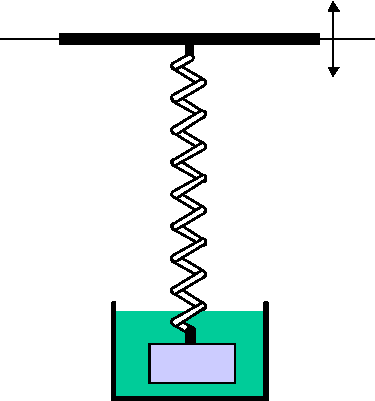
\includegraphics[width=\columnwidth, angle=90, origin=c]{images/spring_dashpot.pdf}}{
$x(t)=$ displacement from rest position\student{\subitem{$x=0 \Rightarrow$ no elastic  restoring force}}
\vfill
Newton's 2$^{nd}$ Law:\[ F = ma \qquad \text{where $a = \ddn{x}{t}{2}$}\]


}
\algn{F&=\text{sum of forces}\\&=\underbrace{\carray{\text{elastic restoring} \\ \text{force}}}_{\student{\carray{\text{Hooke's Law}\\=-kx }}} + \underbrace{\text{drag force}}_{\student{\carray{\text{opposes motion}\\ =-\beta\dd{x}{t}}}} + \quad \underbrace{\text{external forces}}_{\carray{\student{f(t)}}}\\
&= \student{-kx - \beta \dd{x}{t} +f(t)} }
}


\slide[Derivation of spring-dashpot ODE:]{
\twomini[.38]{.25}{.65}{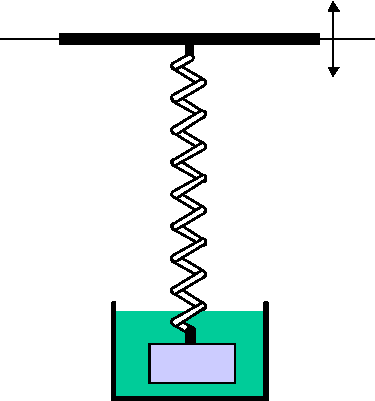
\includegraphics[width=\columnwidth, angle=90, origin=c]{images/spring_dashpot.pdf}}{
$x(t)=$ displacement from rest position\subitem{$x=0 \Rightarrow$ no elastic  restoring force}
\vfill
Newton's 2$^{nd}$ Law:\[ F = ma \qquad \text{where $a = \ddn{x}{t}{2}$}\]


}
\algn{F&=-kx - \beta \dd{x}{t} +f(t) &
\student{\Rightarrow m \ddn{x}{t}{2}} &\student{= -kx - \beta \dd{x}{t} +f(t)}}

\student{\[\boxed{ m x\pp + \beta x\p  + kx=  f(t) }\]
\vfill
With $f(t)=0$ (no external forcing) we get an ODE of the form \[ay''+by'+cy=0\]
}
}


\subsection{Equivalent applications}

\slide[Torsional motion of a weight on a twisted shaft:]{
\twomini{.32}{.65}{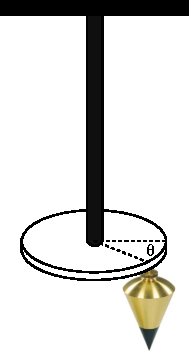
\includegraphics[width=\columnwidth]{images/twisted_shaft.pdf}}{
\vfill\[ I\ddn{\theta}{t}{2} +c \dd{\theta}{t} + k\theta = T(t)\]\vspace*{\fill}
}
}

\slide[L-R-C series circuits:]{
\twomini{.45}{.55}{
\begin{circuitikz} \draw
       (0,-1.5)   to[vsourcesin, l=\textcolor{black}{$E(t)$}] (0,1.5)
	[black] -- (0.5,1.5)
        to[L, l=$L$, black] (1.5,1.5) -- (2.5,1.5)
        to[C, l=$C$, black] (2.5,0) -- (2.5,-1.5)
        to[R, l=$R$, black] (.5,-1.5) -- (0,-1.5) ;
    \end{circuitikz}
}{\vfill
Q=charge on capacitor\\~\\
$\dd{Q}{t}$=current in circuit\\~\\
$E(t)$ = applied voltage\\
\vfill
Kirchoff's Laws:
\[ L\ddn{Q}{t}{2} +R \dd{Q}{t} + \frac1CQ = E(t)\]\vspace*{\fill}
}
}

\slide[Small oscillations of a pendulum:]{
\twomini{.45}{.55}{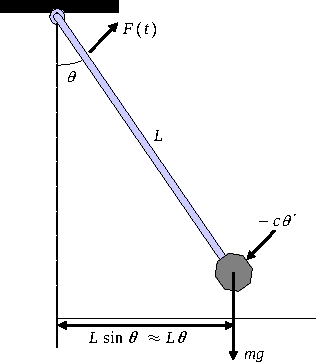
\includegraphics[width=\columnwidth]{images/pendulum.pdf}}{
\vfill\[ mL^2\ddn{\theta}{t}{2}=-cL \dd{\theta}{t} -mgL\theta + F(t) \]\vspace*{\fill}
}
}

\slide[Equivalence of Problems]{
These 4 physical systems are modelled identically by:\[ay\pp+by\p+cy=f(t)\]
\vfill
Constants have different physical meaning (\& units)
\small\vfill
\begin{tabular}{|>{\centering}m{2cm}|>{\centering}m{2cm}|>{\centering}m{2cm}|>{\centering}m{2cm}|>{\centering}p{2cm}|}
\hline 
\textbf{System} & \textbf{a} & \textbf{b} & \textbf{c} & \textbf{f(t)}\tabularnewline
\hline 
\hline 
\textbf{Spring Dashpot} & Mass & Damping Coeff. & Spring Constant & Applied Force\tabularnewline
\hline 
\textbf{Pendulum} & Mass x (Length)$^{2}$ & Damping x Length & Gravitational Moment & Applied Moment\tabularnewline
\hline 
\textbf{Series Circuit} & Inductance & Resistance & Capacitance$^{-1}$ & Imposed Voltage\tabularnewline
\hline 
\textbf{Twisted Shaft} & Moment of Inertia & Damping & Elastic Shaft Constant & Applied Torque\tabularnewline
\hline 
\end{tabular}

}

\subsection{The characteristic polynomial}

\slide[Roots of the characteristic equation (polynomial)]{\vspace{-2em}
\algn{ay''+by'+cy&=0 &\text{guess: } y&=e^{rt}\\
ar^2e^{rt}+bre^{rt}+ce^rt&=0 &\Rightarrow \underbrace{ar^2+br+c}_{\text{char. poly.}}&=0 }

\[r=r_{1,2}=\frac{-b\pm\sqrt{b^2-4ac} }{2a}\]
Three main cases:\student{
\enum{\item Two distinct real roots: $\underbrace{b^2-4ac}_{\text{discriminant}}>0$ \vfill
\item Repeated real roots: discriminant $= 0$ \vfill \item Complex conjugate roots: discriminant $<0$}}
}

\slide[Case 1:  distinct real roots]{
\[y_h(t)=c_1e^{r_1 t} + c_2 e^{r_2 t}; \qquad r_{1,2}=\frac{-b\pm\sqrt{b^2-4ac} }{2a}\] 
 Two major subcases:
\student{\enum{
\item $ac>0$ :\vfill
 Both roots have the same sign.\vfill
$y_1$ and $y_2$ both grow or decay exponentially.
\vfill
\item $ac<0$:
\vfill
The two roots have opposite sign.
\vfill
One solution grows exponentially, the other decays exponentially.

}}


}




\slide[Qualitative Behaviour: distinct real roots]{\vspace{-1em}
Sum of real exponential functions, three subcases:\vfill
\student{
\enum{
\item All positive roots, $0<\textcolor{blue}{r_1}<\textcolor{red}{r_2}$.\\
\tikzplot{.1}{4}{.1}{1.25}{t}{}{
\draw[red ,domain=0:4, samples=120,  thick] plot ({\x}, {0.01*exp(2*\x)});
\draw[blue ,domain=0:4, samples=120,  thick] plot ({\x}, {0.01*exp(\x)});
}
\vfill
\item  Mixed roots, $\textcolor{blue}{r_1}<0<\textcolor{red}{r_2}$.\\
\tikzplot{.1}{4}{.1}{1.25}{t}{}{
\draw[blue ,domain=0:4, samples=120,  thick] plot ({\x}, {1*exp(-2*\x)});
\draw[red ,domain=0:4, samples=120,  thick] plot ({\x}, {0.05*exp(\x)});
}
\vfill
\item All negative roots,  $\textcolor{blue}{r_1}<\textcolor{red}{r_2}<0$.
\\
\tikzplot{.1}{4}{.1}{1.25}{t}{}{
\draw[red ,domain=0:4, samples=120,  thick] plot ({\x}, {exp(-1*\x)});
\draw[blue ,domain=0:4, samples=120,  thick] plot ({\x}, {exp(-2*\x)});
}
}
}
}


\subsection{Case 2: repeated root}

\slide[Case 2: Repeated real root ($r_1=r_2=r$) \hfill $y_h=c_1y_1 + c_2y_2$]{
Straighforward solution \[y_1=e^{rt}\]  with \[r = \frac{-b\pm\sqrt{b^2-4ac} }{2a} = \frac{-b}{2a}\]
We need another solution that is linearly independent of $y_1$
\student{
\vfill

\vfill
Lets try \[y_2=q(t) y_1(t)\]
Unique choice \[q(t)=Ct \qquad \Rightarrow \qquad y_2(t) = te^{rt}\]
}
}
\slide[Proof that $y_2=te^{rt}$]{\vspace{-2.5em}
\[ay\pp + by\p+cy=0 \qquad \text{with } b^2-4ac=0\quad \Rightarrow \quad r_{1,2}=r=\frac{-b}{2a} \]
\centerline{$$}\vspace{-1.75em}
\algn{\text{Try: } y_2 &= q(t)e^{rt}, \quad 
y_2\p = q'e^{rt}+rqe^{rt} \\
y_2\pp &= q''e^{rt} + 2rq'e^{rt}+ r^2qe^{rt} 
\intertext{plug these into the ODE}
&a\left(  q''e^{rt} + 2rq'e^{rt}+ r^2qe^{rt}  \right) + b \left( q'e^{rt}+rqe^{rt}\right) + c q e^{rt} = 0 \\
& a q''e^{rt} +\left( 2ar +b \right)q'e^{rt} +\underbrace{ (ar^2+br+c)}_{\text{char. poly.}=0}qe^{rt} =0 
\intertext{sub in $r=\frac{-b}{2a}$} 
&aq''e^{rt} +\underbrace{\left( \cancel{2a}\frac{-b}{\cancel{2a}} +b \right)}_{0}e^{rt} =0 \\
& aq''e^{rt} = 0 \quad \Rightarrow  \quad  q''=0 \quad \Rightarrow  \quad  q(t) = Ct+D }
$D=0$ due to linear independence between $y_2$ and $y_1$
}

\slide[Checking for linear independence when $r_1=r_2=r$]{
Both $y_1=e^{rt}$ and $y_2=te^{rt}$ are solutions.
\vfill
$W(y_1,y_2)(t)=y_1y_2\p -y_1\p y_2$?
\student{\algn{W&=e^{rt}\left(rte^{rt} + e^{rt}\right)-re^{rt}te^{rt}\\
&=\cancel{rte^{2rt}}+e^{2rt}-\cancel{rte^{2rt}}\\
&=e^{2rt}  \neq 0 }
\vfill
$y_1$ and $y_2$ are linearly independent!
\vfill
General solution: $y_h = c_1e^{rt} + c_2 te^{rt}$

}
}

\slide[Solve the IVP: $y\pp+4y\p+4y=0 \qquad \rarray{y(0)=2\\y\p(0)=0}$ ]{

\student{\algn{r_{1,2} &= \frac{-4\pm\sqrt{16-4\cdot 4}}{2} = \frac{-4\pm 0}{2} =,-2\\
y_h&=c_1e^{-2t}+c_2te^{-2t} \intertext{initial conditions:}
y(0)=2&=c_1\\
y\p(0)=0&=-2c_1 + c_2(e^{-2t}-2te^{-2t})\evalat{t=0}{} \\&= -4 +c_2 \qquad \Rightarrow \qquad c_2=4\\
\Aboxed{y(t) &= 2 e^{-2t} + 4 t e^{-2t}}
}
}

}

\settoggle{covered}{false}
\subsection{Case 3: complex conjugate roots}
\slide[Review: Complex Numbers]{
\twomini[.9]{.5}{.5}{
Square root of a negative number:
\vfill
Suppose $w>0$
\student{
\algn{\ucover{\sqrt{-w}} & \ucover{=} i\sqrt{w}\\
i&=\text{imaginary unit}\\\\
i \times i &= -1}
}
\vspace{4em}
}{
Suppose $a,b\in \mathbb{R}$\vfill
Complex Number: $z=a+ib$\\
Complex Conjugate: $\bar{z} =a-ib $

\student{\algn{\ucover{\frac{z+\bar{z}}{2}} & \ucover{=}  \frac{2a}{2}\; =  a = \text{Re}(z)\in \mathbb{R}\qquad \\ \\
\ucover{\frac{z-\bar{z}}{2i}} & \ucover{=} \frac{2ib}{2i}=  b = \text{Im}(z) \in \mathbb{R}\qquad
}}

\vspace{3em}
}

}
\slide[Case 3: Complex roots ($b^2-4ac<0$ )  \hfill $y_h=c_1y_1 + c_2y_2$]{
Roots are given by:\algn{r_1&=\alpha + i \beta & \text{where } i =\sqrt{-1} \\
r_2&=\alpha - i \beta}
\student{\vspace{-.75em}\[\alpha = \frac{-b}{2a},\qquad \beta =\frac{\sqrt{4ac-b^2}}{2a}\]}\vfill
The two functions $y_1=e^{(\alpha +i\beta )t}$ \& $y_2=e^{(\alpha  - i\beta) t}=\bar{y}_1$ are solutions.\vfill
\student{What is the exponential of a complex number?\vfill Euler's formula:\[e^{\pm i \alpha} = \cos \alpha \pm i \sin \alpha\]}

}
\settoggle{covered}{false}
\slide{\vspace{-1.5em}
\student{
\algn{y_{1,2}=e^{(\alpha  \pm i\beta ) t} &= e^{\alpha t} e^{\pm i \beta t} \\ &=  \underbrace{e^{\alpha t}}_{\text{Real}} \underbrace{[\underbrace{ \cos(\beta t)}_{\text{Real}} \pm\underbrace{ i \sin (\beta t)}_{\text{Imaginary}}]}_{\text{Complex Conjugates}}&y_1=\bar{y}_2&}

We want purely real solutions
\vfill
\algn{\tilde{y}_1 & = \frac{y_1+y_2}{2}=\text{Re}(y_1) =e^{\alpha t} \cos(\beta t)  \in \mathbb{R} \\
\tilde{y}_2&=\dfrac{y_1-y_2}{2i}=\text{Im}(y_1)=e^{\alpha t} \sin (\beta t) \in \mathbb{R}
}
\vfill
}
}

\slide[Complex roots ($r_{1,2}=\alpha\pm i \beta$)]{
The functions $y_1=e^{\alpha t} \cos (\beta t)$ and $y_2=e^{\alpha t} \sin (\beta t)$ are linearly independent real solutions. 

\student{
\vfill
Sketch the two functions if you are not convinced.\vfill
General solution: $y_h = c_1e^{\alpha t} \cos (\beta t) + c_2 e^{\alpha t} \sin (\beta t)$}

}

\slide[Find the general solution to: $y\pp+6y=0 $ ]{
\student{\algn{r_{1,2} &= \frac{\pm\sqrt{-4\cdot 6}}{2} = \pm \sqrt{-6} = \pm i\sqrt{6} \\
y_h&=c_1 \cos \left(\sqrt{6}t\right) + c_2 \sin\left( \sqrt{6}t\right) 
}
}
}

\slide[Solve the IVP: $y\pp+2y\p+5y=0 \qquad \rarray{y(0)=1\\y\p(0)=-1}$ ]{
\student{\algn{r_{1,2} &= \frac{-2\pm\sqrt{4-4\cdot 5}}{2} = \frac{-2\pm \sqrt{-16}}{2}=-1\pm \frac{\sqrt{16}}{2} i = -1\pm 2i \\
y_h&=e^{-t} \left(c_1 \cos \left(2t\right) + c_2 \sin\left( 2t\right) \right)\intertext{initial conditions:}
y(0)=1&=c_1\\
y\p(0)=-1&= -c_1+ \left(-2 c_1 \sin \left(0\right) + 2 c_2 \cos\left( 0 \right) \right) = -c_1+2c_2\\
-1&=-1+2c_2  \qquad \Rightarrow  \qquad  c_2=0\\\\
\Aboxed{y(t) &= e^{-t}\cos (2t)}
}
}
}

\slide[Qualitative Behaviour: complex roots]{\vspace{-1em}
Three subcases:

\student{
\enum{
\item  $\alpha < 0\quad\Rightarrow\quad$ Exponentially decaying oscillations.
\tikzplot{.1}{10}{.75}{.75}{t}{}{
\draw[domain=0:10, samples=300,  thick, color=blue] plot ({\x}, {0.75*exp(-.2*\x)*sin(360*\x)});
\draw[domain=0:10, samples=300,  thick, color=red] plot ({\x}, {0.75*exp(-.2*\x)*cos(360*\x)});
\draw[domain=0:10, samples=300,  thick, dashed] plot ({\x}, {0.75*exp(-.2*\x)})  node[left, xshift=-4cm, yshift=.4cm]{$e^{\alpha t}$};
\draw[domain=0:10, samples=300,  thick, dashed] plot ({\x}, {-0.75*exp(-.2*\x)}) node[left, xshift=-4cm, yshift=-.4cm]{$-e^{\alpha t}$};
}
\vfill
\item   $\alpha = 0 \quad\Rightarrow\quad$ Sustained periodic oscillations.
\tikzplot{.1}{10}{.75}{.75}{t}{}{
\draw[domain=0:10, samples=300,  thick, color=blue] plot ({\x}, {.72*sin(360*\x)});
\draw[domain=0:10, samples=300,  thick, color=red] plot ({\x}, {.72*cos(360*\x)});
}
\vfill
\item  $\alpha > 0\quad\Rightarrow\quad$ Exponentially growing oscillations.
\tikzplot{.1}{10}{.75}{.75}{t}{}{
\draw[domain=0:10, samples=300,  thick, color=blue] plot ({\x}, {0.1*exp(.2*\x)*sin(360*\x)});
\draw[domain=0:10, samples=300,  thick, color=red] plot ({\x}, {0.1*exp(.2*\x)*cos(360*\x)});
\draw[domain=0:10, samples=300,  thick, dashed] plot ({\x}, {0.1*exp(.2*\x)})  node[left, xshift=-4cm, yshift=-.15cm]{$e^{\alpha t}$};
\draw[domain=0:10, samples=300,  thick, dashed] plot ({\x}, {-0.1*exp(.2*\x)}) node[left, xshift=-4cm, yshift=.15cm]{$-e^{\alpha t}$};
}
}
}
}

\slide[Summary]{
\itmz{
\item For homogeneous linear constant coeffiecient ODEs:
\subitem{Pick an ansatz (e.g., $e^{rt}$) \item Write down the characteristic equation
\item Find the roots \subitem{If you don't have enough functions, make a new one by multiplying by $t$}}
\vfill
\item Write down the general solution according to the roots
\subitem{ Real and distinct $\Rightarrow y_h = c_1e^{r_1t} + c_2 e^{r_2t}$ }
\subitem{ Real and repeated $\Rightarrow y_h = c_1e^{rt} + c_2 te^{rt} $ }
\subitem{ Complex $\Rightarrow y_h= c_1e^{\alpha t} \cos (\beta t) + c_2 e^{\alpha t} \sin (\beta t)$  \hfill with $r_{1,2} = \alpha\pm i\beta$}
\vfill
\item Fit the constants $c_1$ and $c_2$ to the initial conditions
}
}


\end{document}